\subsection{Основные методики обработки температурных кинетик}
Для расчёта коэффициента оптического поглощения из экспериментальных данных о кинетике температуры с использованием уравнения теплового баланса~\cref{eq:balance_equation} применяются три основные методики. Экспоненциальная и импульсная методики основаны на аппроксимации участков нагрева образца лазерным излучением и его остывания, соответственно; градиентная методика основана на определении разности производных разогрева на участках нагрева и остывании при одной и той же величине разогрева.

\nomenclature[N]{$I, E, G$~[\si{\kelvin\per\second}]}{Тепловой источник, определённый по импульсной, экспоненциальной, градиентной методикам соответственно}

\subsubsection{Экспоненциальная методика}
Поскольку решением балансного уравнения являются экспоненциальные зависимости, представляется возможным аппроксимировать экспериментальные данные для перегрева кристалла относительно комнатной температуры $\Delta T := T(t) - T_a$ следующей формулой:
\begin{equation}
	f(t) = A + Be^{-Ct}
	\label{eq:exp_fit}
\end{equation}

при нагреве ($t < t_0$) и остывании ($t > t_0$) соответственно. Сравнивая аппроксимирующую функцию (\ref{eq:exp_fit}) с решением уравнения теплового баланса (\ref{eq:balance_equation_solution}), получаем выражение для усреднённого теплового источника:

\begin{equation}
	E = A_{\text{exp}}C_{\text{exp}} = \overline{Q},
	\label{eq:barq_exp}
\end{equation}


Отметим, что при аппроксимации кинетики остывания данная методика будет совпадать с импульсной, поэтому далее под экспоненциальной методикой мы будем понимать аппроксимацию участка кинетики, отвечающего за нагрев образца лазерным излучением. Величины, полученные аппроксимацией кинетики нагрева, далее обозначены индексом <<exp>>, а кинетики остывания --- индексом <<puls>>.

\nomenclature[N]{$\varkappa$~[\si{\watt\per(\meter\ensuremath{\cdot}\kelvin)}]}{Коэффициент теплопроводности}

Применение методики ограничено в случае низкого коэффициента теплопроводности образца, вернее, в случае малого числа Био, характеризующего однородность распределения температуры по образцу \( b = \frac{hR}{\varkappa} \). Здесь \( R \) — характерные линейные размеры образца, \( \varkappa \) — коэффициент теплопроводности.   Это обусловлено тем, что кинетики нагрева будут отличаться при разных положениях термодатчика относительно лазерного пучка.






\subsubsection{Импульсная методика}
В импульсной методике требуется произвести экстраполяцию кинетики охлаждения до середины времени включения лазера $t=t_0/2$ и использовать экстраполированную температуру для расчёта поглощения.

Согласно (\ref{eq:balance_equation_solution}), значение экстраполированной по кинетике остывания температуры в этот момент времени составляет

\begin{equation}
	T(t_0/2) = T_a + \dfrac{\overline{Q}}{\Gamma}\left(1-\exp{(-\Gamma t_0)}\right)\exp{(\Gamma t_0/2)} = T_a + 2\dfrac{\overline{Q}}{\Gamma}\sinh{\left(\Gamma t_0 / 2\right)},
	\label{eq:T05}
\end{equation}

Отсюда получаем выражение для среднего теплового источника, определяемого по результатам экстраполяции кинетики остывания:

\begin{equation}
	I = \frac{C_{\text{puls}}f(t_0/2)}{2\sinh(C_{\text{puls}}t_0/2)} = \overline{Q}.
	\label{eq:barq_puls}
\end{equation}



\begin{figure}[h!]
	\centering
	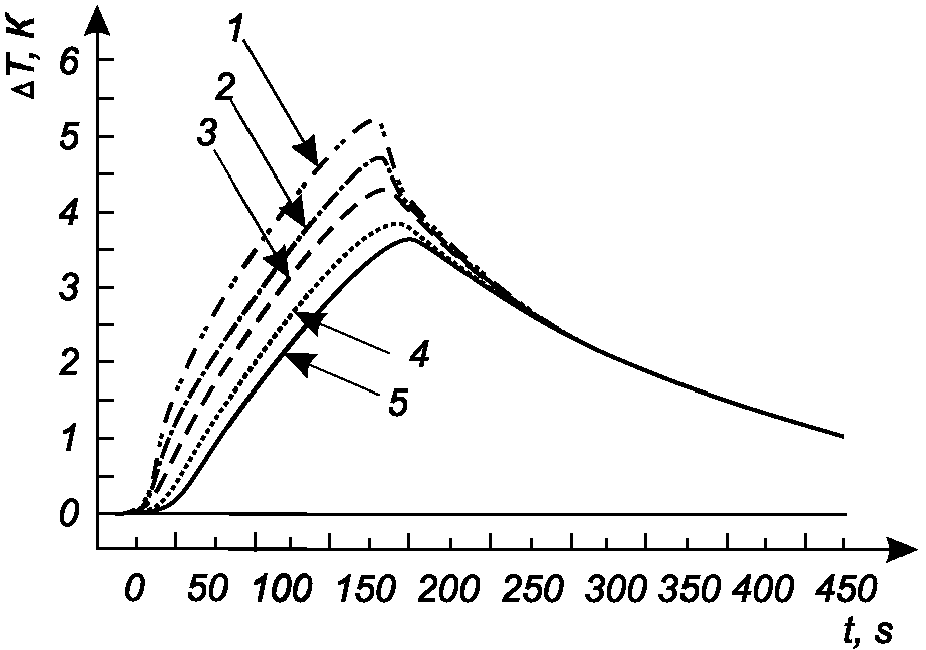
\includegraphics[width=0.7\linewidth]{Dissertation/images/review/conductivity}
	\caption{Влияние конечной теплопроводности. Кривые 1, 2, 4, 5 соответствуют различным точкам расположения датчика температуры относительно лазерного пучка: 6, 7, 9, 12 мм соответственно. Кривая 3 соответствует модели с бесконечной теплопроводностью~\cite{iso}.}
	\label{fig:cond}
\end{figure}

В области охлаждения все отличия по теплопроводности, связанные с зависимостью кинетики от положения термодатчика, сходятся к одной кривой, поскольку при остывании градиент температуры внутри материала успевает выравняться значительно быстрее, чем происходит теплообмен с окружающей средой, см. рис.~\cref{fig:cond}. Это означает, что кинетика остывания на поздних стадиях становится универсальной и не зависит от начального распределения температуры, созданного в момент нагрева. Данное свойство делает импульсная методика перспективным для определения коэффициента оптического поглощения при низких значениях числа Био.

\subsubsection{Градиентная методика}


В градиентной методике анализируется разность производных температуры в моменты времени, соответствующих одной и той же температуре \( T_0 \) при нагреве и охлаждении:


\begin{equation}
	G = \frac{d T}{d t} \bigg|_{t < t_0, T = T_0} - \frac{d T}{d t} \bigg|_{t > t_0, T = T_0}.
	\label{eq:barq_grad}
\end{equation}


Из (\ref{eq:barq_grad}) следует, что при неизменной температуре окружающей среды \( G \equiv \overline{Q} \).

\begin{figure}[h]
	\centering
	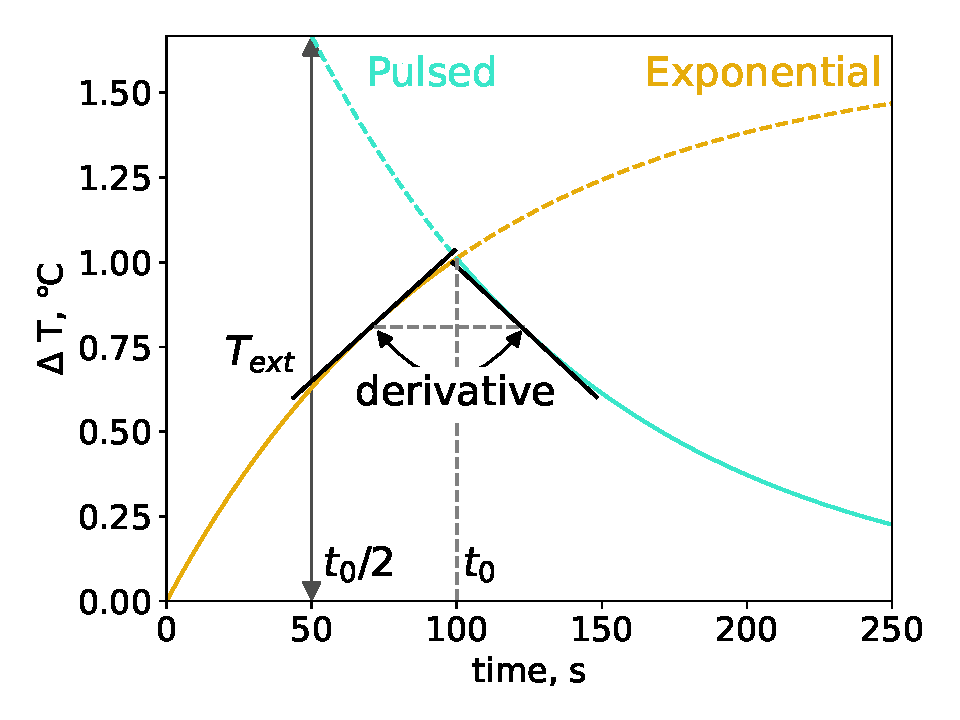
\includegraphics[width=0.8\textwidth]{Dissertation/images/review/illustrative_example}
	\caption{Иллюстрация методик обработки температурной кинетики}
	\label{fig:illustrativeexample}
\end{figure}

На рис.~\cref{fig:illustrativeexample} проиллюстрировано использование всех трёх методик для обработки температурной кинетики.

Конечная теплопроводность образца (малое число Био) вносит погрешности во все рассмотренные методики измерений, однако наибольшее влияние она оказывает на градиентный метод \cite{Meja1997}. Это связано с выраженной зависимостью величины $G$ от расположения внешнего термодатчика. Именно данное ограничение послужило причиной исключения градиентной методики из стандарта ISO~11551 в 2003~году \cite{iso_old}. Тем не менее, только эта методика обеспечивает возможность регистрации временной динамики коэффициента оптического поглощения, что, например, делает его подходящим инструментом для изучения процессов деградации оптических элементов под воздействием лазерного излучения \cite{Zotov2023}.

Помимо упомянутых выше, в различных работах \cite{willamowski1999standardisierbare} представлены такие методики, как, например, интегральный и метод отклика (Responseverfahren). 

Подробный анализ погрешностей импульсной и градиентной методик выполнен в работе~\cite{arenberg2000error}. Автор показывает, что при использовании импульсного метода основной вклад в неопределённость измерения коэффициента поглощения вносит погрешность измерения мощности лазера, тогда как вклады неопределённости массы, теплоёмкости, температуры и времени пренебрежимо малы. Для градиентного метода дополнительными значимыми источниками погрешности становятся погрешности определения скоростей нагрева и охлаждения. В работе рекомендуется по возможности использовать импульсный метод как обеспечивающий меньшую неопределённость и более высокую воспроизводимость измерений по сравнению с градиентным. Однако влияние внешних факторов на точность определения коэффициента оптического поглощения, таких, как непостоянство температуры окружающей среды и коэффициента теплоотдачи, в работе не рассматривалось.
